\documentclass[conference,a4paper]{IEEEtran}
\pdfminorversion=6

% =========================================================
% Packages
% =========================================================
\usepackage[margin=0.75in]{geometry}
\usepackage{times}
\usepackage{graphicx}
\usepackage{booktabs}
\usepackage{multirow}
\usepackage{amsmath,amssymb}
\usepackage{algorithm}
\usepackage{algpseudocode}
\usepackage{subcaption}
\usepackage{xcolor}
\usepackage{url}
\usepackage{cite}
\usepackage[section]{placeins}
\usepackage{tikz}
\usepackage[hidelinks]{hyperref}
\usetikzlibrary{arrows.meta,positioning}

\renewcommand{\topfraction}{0.95}
\renewcommand{\textfraction}{0.05}
\renewcommand{\floatpagefraction}{0.85}

% =========================================================
% Paper metadata
% =========================================================
\title{
HN-SARD: Hard-Negative Scale-Aware Region Distillation\\
for Nine-Dash Line Detection in Cartographic Content
}

\author{
Anonymous Authors
}

\date{}

\begin{document}
\maketitle

% =========================================================
% Abstract: ~0.15 page
% =========================================================
\begin{abstract}
Nine-dash line detection is a challenging visual moderation problem because the target is often tiny, thin, fragmented, and visually similar to benign cartographic structures such as coastlines, rivers, dashed boundaries, and grid lines.
In this paper, we introduce a benchmark for nine-dash line detection with positive samples, in-domain negative maps, and out-domain negative images.
To address both missed tiny objects and false positives on visually similar clean maps, we propose HN-SARD, a Hard-Negative Scale-Aware Region Distillation framework.
HN-SARD uses Faster R-CNN as the student detector and a frozen DINOv2 visual foundation model as a region-level teacher.
It combines scale-aware positive region distillation with online hard-negative contrastive distillation.
Beyond standard object-level AP, we evaluate models using moderation-oriented metrics, including image-level AUROC, FPR@95TPR, and in-domain false positive rate.
Experiments show that HN-SARD improves the high-recall, low-false-positive trade-off required for sensitive cartographic content moderation.
\end{abstract}

% =========================================================
% 1. Introduction: ~0.75--0.85 page
% =========================================================
\section{Introduction}

Nine-dash line imagery can appear in digital maps, educational materials, social media posts, videos, and document screenshots.
Automatically detecting such visual content is important for moderation systems, but the task is not a standard object detection problem.
The target pattern is usually thin, discontinuous, low-contrast, and may occupy only a small fraction of the image.

A key difficulty is that benign cartographic content can contain visually similar structures.
Coastlines, rivers, administrative borders, dashed routes, grid lines, and contour lines may resemble parts of the nine-dash line.
Therefore, a practical detector must not only detect violations but also avoid falsely flagging clean maps.

Existing detection pipelines often emphasize object-level AP.
However, for visual moderation, deployment risk is also determined by image-level false alarms, especially on in-domain negative maps.
A detector with slightly higher AP may still be less useful if it produces many false positives on clean cartographic images.

In this work, we revisit nine-dash line detection from a moderation-oriented perspective.
We construct a benchmark containing positive images, in-domain negative maps, and out-domain negative images.
We then propose HN-SARD, a Hard-Negative Scale-Aware Region Distillation framework designed to improve small/thin object detection and reduce false positives on hard negative regions.

Our contributions are threefold:
\begin{itemize}
    \item We introduce a benchmark for nine-dash line detection with explicit positive, in-domain negative, and out-domain negative partitions.
    \item We propose HN-SARD, which distills region-level knowledge from a frozen DINOv2 teacher using scale-aware positive region distillation and online hard-negative contrastive distillation.
    \item We evaluate detectors using both object-level metrics and moderation-oriented metrics, including FPR@95TPR, in-domain FPR, and FROC analysis.
\end{itemize}

% =========================================================
% 2. Related Work: ~0.45--0.55 page
% =========================================================
\section{Related Work}

\paragraph{Small and thin object detection.}
Detecting small and elongated objects remains difficult because such objects provide weak spatial and semantic signals.
Two-stage detectors with feature pyramids are often used for small-object scenarios because they allow region-level feature extraction and proposal refinement~\cite{ren2015faster,lin2017feature}.

\paragraph{Knowledge distillation for object detection.}
Knowledge distillation transfers information from a teacher model to a student detector~\cite{hinton2015distilling}.
Prior work has explored feature-level, logit-level, relation-level, and region-level distillation for object detection~\cite{wang2019distilling}.
In this work, we focus on region-level distillation because the nine-dash line is localized and visually subtle.

\paragraph{Visual foundation models as teachers.}
Self-supervised visual foundation models such as DINOv2 learn strong visual representations without task-specific labels~\cite{oquab2024dinov2}.
We use DINOv2 as a frozen visual teacher, not as a vision-language model.
Instead of applying it to the full image, we extract context-aware region crops to make tiny and thin objects more visible to the teacher.

\paragraph{Hard negative mining and contrastive learning.}
Hard negative mining improves discriminative learning by focusing on confusing background regions~\cite{shrivastava2016training}.
Contrastive learning further encourages separation between positive and negative representations~\cite{oord2018representation}.
HN-SARD combines these ideas by contrasting positive nine-dash line regions against online hard-negative proposals.

\paragraph{Moderation-oriented evaluation.}
Visual moderation systems are judged not only by detection accuracy but also by false-alarm behavior at high recall.
For cartographic content, in-domain false positives are especially important because clean maps can contain many target-like structures.
This motivates image-level metrics and FROC analysis in addition to standard object-level AP.

% =========================================================
% 3. Dataset: ~0.75--0.85 page
% =========================================================
\section{Dataset}

\subsection{Benchmark Design}

We construct a benchmark for nine-dash line detection with three major groups:
\begin{itemize}
    \item \textbf{Positive images}: images containing nine-dash line instances.
    \item \textbf{In-domain negatives}: cartographic or geographic images without nine-dash line but containing visually similar structures.
    \item \textbf{Out-domain negatives}: general images outside the cartographic domain.
\end{itemize}

\subsection{Annotation Protocol}

We annotate each visible nine-dash line instance with a bounding box and use a single object category.
For fragmented instances, the annotation covers the visible extent of the target pattern rather than each small dash independently.
Negative images are kept without object boxes.
Ambiguous cases are reviewed conservatively, since inconsistent labels would directly affect both object-level AP and image-level false-positive metrics.

\subsection{Dataset Split}

We use a stratified image-level split to preserve the distribution of positive images, negative images, and object scales across train, validation, and test sets.
Table~\ref{tab:dataset_split} summarizes the split.

\begin{table}[!htbp]
\centering
\caption{Dataset composition by split. In-domain negatives are cartographic images that do not contain the target pattern, while out-domain negatives are non-cartographic or weakly related images.}
\label{tab:dataset_split}
\resizebox{\linewidth}{!}{
\begin{tabular}{lrrrrr}
\toprule
Split & Pos. & In-Dom. Neg. & Out-Dom. Neg. & Total & Objects \\
\midrule
Train & 1,642 & 2,048 & 1,451 & 5,141 & 1,837 \\
Val   & 352   & 439   & 311   & 1,102 & 402   \\
Test  & 351   & 439   & 311   & 1,101 & 397   \\
\bottomrule
\end{tabular}
}
\end{table}

\subsection{Object Scale Distribution}

Because nine-dash line instances can be tiny and fragmented, we report performance by object scale.
Table~\ref{tab:test_scale} shows the scale distribution in the test set.

\begin{table}[!htbp]
\centering
\caption{Object scale distribution in the test set. Tiny instances are scarce, so we report confidence intervals and qualitative analysis for this group.}
\label{tab:test_scale}
\begin{tabular}{lrr}
\toprule
Size Group & Images & Objects \\
\midrule
Large  & 201 & 202 \\
Medium & 93  & 104 \\
Small  & 43  & 67  \\
Tiny   & 14  & 24  \\
\bottomrule
\end{tabular}
\end{table}

\noindent
Additional dataset statistics, including bbox width, bbox height, bbox area ratio, and UMAP/t-SNE visualizations, are provided in Appendix~\ref{app:dataset_details}.
\FloatBarrier

% =========================================================
% 4. Method: ~1.35--1.50 pages
% =========================================================
\section{Method}

\subsection{Overview}

HN-SARD is built on Faster R-CNN with an R50-FPN backbone~\cite{ren2015faster,lin2017feature}.
The student detector is trained using the standard detection loss and two additional distillation objectives:
scale-aware positive region distillation and online hard-negative contrastive distillation.

Figure~\ref{fig:architecture} summarizes the training pipeline.
The DINOv2 branch is used only during training; inference uses the student detector alone.

\begin{figure}[!t]
\centering
\resizebox{\linewidth}{!}{
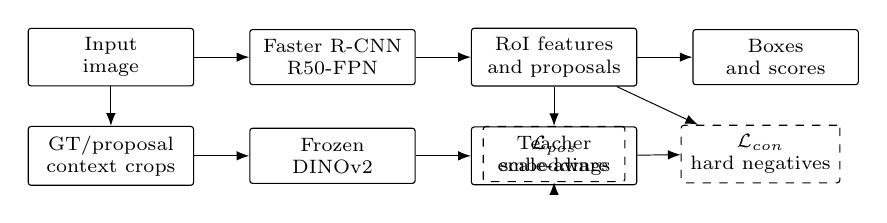
\begin{tikzpicture}[
    node distance=5mm and 7mm,
    block/.style={draw, rounded corners=1pt, align=center, minimum width=21mm, minimum height=7mm, font=\scriptsize},
    loss/.style={draw, dashed, rounded corners=1pt, align=center, minimum width=18mm, minimum height=7mm, font=\scriptsize},
    arrow/.style={-Latex, line width=0.35pt}
]
\node[block] (img) {Input\\image};
\node[block, right=of img] (student) {Faster R-CNN\\R50-FPN};
\node[block, right=of student] (roi) {RoI features\\and proposals};
\node[block, right=of roi] (pred) {Boxes\\and scores};

\node[block, below=of img] (crop) {GT/proposal\\context crops};
\node[block, right=of crop] (teacher) {Frozen\\DINOv2};
\node[block, right=of teacher] (temb) {Teacher\\embeddings};

\node[loss, below=of roi] (lpos) {$\mathcal{L}_{pos}$\\scale-aware};
\node[loss, right=of lpos] (lcon) {$\mathcal{L}_{con}$\\hard negatives};

\draw[arrow] (img) -- (student);
\draw[arrow] (student) -- (roi);
\draw[arrow] (roi) -- (pred);
\draw[arrow] (img) -- (crop);
\draw[arrow] (crop) -- (teacher);
\draw[arrow] (teacher) -- (temb);
\draw[arrow] (roi) -- (lpos);
\draw[arrow] (temb) -- (lpos);
\draw[arrow] (roi) -- (lcon);
\draw[arrow] (temb) -- (lcon);
\end{tikzpicture}
}
\caption{
HN-SARD training architecture. The student detector provides RoI features and proposals, while a frozen DINOv2 teacher embeds context crops for positive region alignment and hard-negative contrastive distillation.
}
\label{fig:architecture}
\end{figure}

The overall objective is:
\begin{equation}
\mathcal{L}
=
\mathcal{L}_{det}
+
\lambda_{pos}\mathcal{L}_{pos}
+
\lambda_{con}\mathcal{L}_{con}.
\label{eq:total_loss}
\end{equation}

\subsection{Detection Loss}

The detection loss follows the standard Faster R-CNN training objective:
\begin{equation}
\mathcal{L}_{det}
=
\mathcal{L}_{rpn-cls}
+
\mathcal{L}_{rpn-reg}
+
\mathcal{L}_{roi-cls}
+
\mathcal{L}_{roi-reg}.
\label{eq:det_loss}
\end{equation}

\subsection{Context-Aware DINOv2 Region Teacher}

For each ground-truth region or selected proposal, we crop the corresponding image region, enlarge it by a context factor $c$, and resize it to the DINOv2 input resolution.
The teacher embedding is extracted as:
\begin{equation}
z_i^T = f_T(\text{crop}_c(g_i)),
\label{eq:teacher_embedding}
\end{equation}
where $f_T$ is the frozen DINOv2 teacher and $g_i$ is the ground-truth box or selected region.

This region-crop strategy is important because applying the teacher to the full image may make tiny nine-dash line instances too small relative to the teacher patch size.

\subsection{Scale-Aware Positive Region Distillation}

For each positive RoI $r_i$, the student embedding is:
\begin{equation}
z_i^S = f_S(r_i),
\label{eq:student_embedding}
\end{equation}
where $f_S$ denotes the student region encoder.

We L2-normalize both student and teacher embeddings:
\begin{equation}
\hat{z}_i^S = \frac{z_i^S}{\|z_i^S\|_2},
\quad
\hat{z}_i^T = \frac{z_i^T}{\|z_i^T\|_2}.
\end{equation}

The positive distillation loss is:
\begin{equation}
\mathcal{L}_{pos}
=
\frac{1}{\sum_{i \in P}\alpha_i}
\sum_{i \in P}
\alpha_i
\left(
1 -
\cos(\hat{z}_i^S,\hat{z}_i^T)
\right),
\label{eq:pos_loss}
\end{equation}
where $P$ is the set of positive regions and $\alpha_i$ is a scale-aware weight.

We use larger weights for smaller objects:
\begin{equation}
\alpha_i =
\begin{cases}
2.0, & \text{tiny},\\
1.5, & \text{small},\\
1.2, & \text{medium},\\
1.0, & \text{large}.
\end{cases}
\end{equation}

The normalization by $\sum_{i \in P}\alpha_i$ prevents the loss magnitude from exploding when a batch contains many small or tiny objects.

\subsection{Online Hard-Negative Mining}

For positive images, hard negatives are proposals with low overlap with ground-truth boxes but high objectness or class confidence:
\begin{equation}
HN = \{r_j \mid \text{IoU}(r_j, G) < \theta_n\}.
\end{equation}

For negative images, we select the top-$K$ proposals according to objectness or class confidence.
These proposals are likely to be confusing background regions such as dashed boundaries, coastlines, rivers, or grid lines.

\subsection{Hard-Negative Contrastive Distillation}

For each positive region $i$, we contrast its student embedding against the teacher embedding of the positive region and the teacher embeddings of hard-negative crops:
\begin{align}
a_i &= \exp\left(\cos(\hat{z}_i^S,\hat{z}_i^T)/\tau\right), \\
b_{ij} &= \exp\left(\cos(\hat{z}_i^S,\hat{h}_j^T)/\tau\right), \\
\mathcal{L}_{con}
&=
-\frac{1}{|P|}
\sum_{i \in P}
\log
\frac{a_i}{a_i + \sum_{j \in HN_i} b_{ij}} .
\label{eq:contrastive_loss}
\end{align}

Here, $h_j^T$ denotes the DINOv2 teacher embedding of a hard-negative crop, $\hat{h}_j^T$ is its L2-normalized form, $HN_i$ is the hard-negative set associated with positive region $i$, and $\tau$ is the temperature.

To avoid noisy negatives in early training, we use a warm-up schedule:
\begin{itemize}
    \item Epochs 1--5: train with $\mathcal{L}_{det}$ and $\mathcal{L}_{pos}$.
    \item From epoch 6 onward: enable $\mathcal{L}_{con}$.
\end{itemize}

% =========================================================
% 5. Experiments: ~1.45--1.65 pages
% =========================================================
\section{Experiments}

\subsection{Implementation Details}

Unless otherwise stated, we use Faster R-CNN R50-FPN as the student detector~\cite{ren2015faster,lin2017feature}.
DINOv2 is frozen during training~\cite{oquab2024dinov2}.
The default context crop factor is $c=2.0$.
For hard-negative mining, we use top-$K=16$ hard negatives per image.
The default temperature is $\tau=0.07$.
All models are trained using the same train/val/test split.

\subsection{Evaluation Metrics}

We report standard object-level metrics:
AP, AP50, AP75, AP$_{tiny}$, AP$_{small}$, AP$_{medium}$, AP$_{large}$, and AR@100, following the COCO-style detection protocol~\cite{lin2014microsoft}.

For moderation-oriented evaluation, we convert detection results into image-level scores:
\begin{equation}
s(I) = \max_{b \in B_I} conf(b),
\end{equation}
where $B_I$ is the set of predicted boxes in image $I$.
We then report image-level AUROC, image-level AP, FPR@95TPR, Recall@FPR=1\%, Recall@FPR=5\%, in-domain FPR, and out-domain FPR.
AUROC follows the standard receiver operating characteristic analysis protocol~\cite{fawcett2006introduction}.

\subsection{Main Comparison}

Table~\ref{tab:main_comparison} compares HN-SARD with standard detectors and prior distillation baselines, including Faster R-CNN~\cite{ren2015faster}, YOLOv10~\cite{wang2024yolov10}, Ultralytics YOLO11~\cite{jocher2024yolo11}, and RT-DETR~\cite{zhao2023rtdetr}.

\begin{table}[!htbp]
\centering
\caption{Main comparison on the test set. HN-SARD is evaluated using both object-level detection metrics and moderation-oriented false-positive metrics.}
\label{tab:main_comparison}
\setlength{\tabcolsep}{2.2pt}
\scriptsize
\resizebox{\linewidth}{!}{
\begin{tabular}{lrrrrrrrrr}
\toprule
Method & AP & AP50 & AP75 & AP$_t$ & AP$_s$ & AP$_m$ & AP$_l$ & FPR95 & FPR$_{in}$ \\
\midrule
Faster R-CNN R50-FPN  & -- & -- & -- & -- & -- & -- & -- & -- & -- \\
Faster R-CNN R101-FPN & -- & -- & -- & -- & -- & -- & -- & -- & -- \\
YOLOv10/YOLOv11      & -- & -- & -- & -- & -- & -- & -- & -- & -- \\
RT-DETR              & -- & -- & -- & -- & -- & -- & -- & -- & -- \\
Old KD               & -- & -- & -- & -- & -- & -- & -- & -- & -- \\
HN-SARD              & -- & -- & -- & -- & -- & -- & -- & -- & -- \\
\bottomrule
\end{tabular}
}
\end{table}

\subsection{Dataset Ablation}

We evaluate the role of negative data by training Faster R-CNN R50-FPN on four data configurations.
This experiment tests whether in-domain negative maps are necessary for reducing false positives on clean cartographic images.

\begin{table}[!htbp]
\centering
\caption{Dataset ablation. In-domain negative data is expected to reduce false positives on visually similar clean maps.}
\label{tab:dataset_ablation}
\resizebox{\linewidth}{!}{
\begin{tabular}{lrrrrr}
\toprule
Training Data & AP & AP50 & FPR$_{in}$ & FPR$_{out}$ & FPR@95TPR \\
\midrule
Positive only                  & -- & -- & -- & -- & -- \\
Positive + out-domain negative & -- & -- & -- & -- & -- \\
Positive + in-domain negative  & -- & -- & -- & -- & -- \\
Positive + both negatives      & -- & -- & -- & -- & -- \\
\bottomrule
\end{tabular}
}
\end{table}
\FloatBarrier

\subsection{Method Ablation}

Table~\ref{tab:method_ablation} analyzes each component of HN-SARD.

\begin{table}[!htbp]
\centering
\caption{Method ablation. $\mathcal{L}_{pos}$ targets region-level alignment, scale-aware weighting emphasizes small objects, and $\mathcal{L}_{con}$ reduces hard-negative false positives.}
\label{tab:method_ablation}
\resizebox{\linewidth}{!}{
\begin{tabular}{lrrrrr}
\toprule
Variant & AP & AP$_{tiny}$ & AP$_{small}$ & FPR$_{in}$ & FPR@95TPR \\
\midrule
Baseline Faster R-CNN      & -- & -- & -- & -- & -- \\
+ $\mathcal{L}_{pos}$      & -- & -- & -- & -- & -- \\
+ Scale-aware weight       & -- & -- & -- & -- & -- \\
+ Hard-negative mining     & -- & -- & -- & -- & -- \\
+ Warm-up strategy         & -- & -- & -- & -- & -- \\
Full HN-SARD               & -- & -- & -- & -- & -- \\
\bottomrule
\end{tabular}
}
\end{table}
\FloatBarrier

\subsection{Context Crop Ablation}

We evaluate the teacher crop factor $c$.
A small crop may lose contextual clues, while an overly large crop may dilute the target signal.

\begin{table}[!htbp]
\centering
\caption{Context crop ablation for the DINOv2 region teacher.}
\label{tab:crop_ablation}
\begin{tabular}{lrrrr}
\toprule
Crop Strategy & AP & AP$_{tiny}$ & AP$_{small}$ & FPR$_{in}$ \\
\midrule
BBox only & -- & -- & -- & -- \\
1.5$\times$ context & -- & -- & -- & -- \\
2.0$\times$ context & -- & -- & -- & -- \\
3.0$\times$ context & -- & -- & -- & -- \\
\bottomrule
\end{tabular}
\end{table}
\FloatBarrier

% =========================================================
% 6. Discussion: ~0.45--0.55 page
% =========================================================
\section{Error Analysis and Discussion}

Figure~\ref{fig:qualitative} compares baseline predictions and HN-SARD predictions.
We focus on five representative cases:
tiny objects, low-contrast instances, fragmented nine-dash lines, in-domain false positives, and hard negative maps.

\begin{figure}[!htbp]
\centering
\IfFileExists{figures/qualitative_results.pdf}{
    \includegraphics[width=\linewidth]{figures/qualitative_results.pdf}
}{
    \fbox{\begin{minipage}[c][0.22\textheight][c]{0.92\linewidth}
    \centering\footnotesize Qualitative results placeholder: input, ground truth, baseline prediction, and HN-SARD prediction.
    \end{minipage}}
}
\caption{
Qualitative comparison between the baseline detector and HN-SARD.
Columns show input image, ground truth, baseline prediction, and HN-SARD prediction.
}
\label{fig:qualitative}
\end{figure}

In moderation settings, AP alone is insufficient.
A detector with higher object-level AP may still be less desirable if it produces many false positives on clean maps.
Therefore, we emphasize FPR@95TPR and in-domain FPR as operational metrics.
HN-SARD is designed for this high-recall, low-false-positive regime.

When two models show a trade-off between AP and in-domain FPR, we prioritize the operating point that preserves high recall while reducing false alarms on clean maps.
This does not imply that AP is unimportant; rather, AP is interpreted together with image-level moderation risk.
The full error taxonomy used for manual inspection is reported in Appendix~\ref{app:error_taxonomy}.

% =========================================================
% 7. Limitations: ~0.20--0.30 page
% =========================================================
\section{Limitations}

Our benchmark contains relatively few tiny instances in the test set.
Therefore, AP$_{tiny}$ should be interpreted with confidence intervals and qualitative analysis.
Second, the use of a DINOv2 teacher increases training cost, although inference uses only the student detector.
Third, this work focuses on image-level detection and does not yet address video-level or PDF-level moderation pipelines.
Finally, nine-dash line annotations can be ambiguous when the symbol is heavily fragmented or partially occluded.

% =========================================================
% 8. Conclusion: ~0.15--0.20 page
% =========================================================
\section{Conclusion}

We presented a benchmark and HN-SARD, a hard-negative scale-aware region distillation framework for nine-dash line detection.
By combining context-aware DINOv2 region teaching, scale-aware positive distillation, and online hard-negative contrastive learning, HN-SARD targets the two central challenges of the task: missed tiny/thin objects and false positives on visually similar clean maps.
Our evaluation highlights the importance of moderation-oriented metrics such as FPR@95TPR and in-domain FPR.

% =========================================================
% References
% =========================================================
\bibliographystyle{IEEEtran}
\bibliography{references}

% =========================================================
% Appendix
% =========================================================
\clearpage
\appendix

\section{Dataset Details}
\label{app:dataset_details}

This appendix provides extended dataset statistics, including:
\begin{itemize}
    \item number of images by source type;
    \item number of objects by split;
    \item bbox width distribution;
    \item bbox height distribution;
    \item bbox area ratio distribution;
    \item object scale distribution;
    \item UMAP/t-SNE visualization of DINOv2 features~\cite{mcinnes2018umap,vandermaaten2008visualizing}.
\end{itemize}

\begin{table}[!htbp]
\centering
\caption{Dataset group summary.}
\label{tab:dataset_group_summary}
\resizebox{\linewidth}{!}{
\begin{tabular}{lrrrr}
\toprule
Group & Images & Positive & Negative & Objects \\
\midrule
Positive & 2,345 & 2,345 & 0 & 2,636 \\
In-domain negative & 2,926 & 0 & 2,926 & 0 \\
Out-domain negative & 2,073 & 0 & 2,073 & 0 \\
\bottomrule
\end{tabular}
}
\end{table}

\begin{table}[!htbp]
\centering
\caption{Bounding-box summary for nine-dash line annotations.}
\label{tab:bbox_summary}
\resizebox{\linewidth}{!}{
\begin{tabular}{lrrrrrr}
\toprule
Class & Count & W Mean & W Med. & H Mean & H Med. & Area Ratio Mean \\
\midrule
nine-dash line & 2,636 & 329.8 & 273.0 & 448.5 & 378.3 & 0.294 \\
\bottomrule
\end{tabular}
}
\end{table}

\begin{figure}[!htbp]
\centering
\IfFileExists{figures/dataset_umap.pdf}{
    \includegraphics[width=\linewidth]{figures/dataset_umap.pdf}
}{
    \fbox{\begin{minipage}[c][0.20\textheight][c]{0.92\linewidth}
    \centering\footnotesize Dataset feature visualization placeholder: positive samples, in-domain negatives, and out-domain negatives.
    \end{minipage}}
}
\caption{
UMAP visualization of DINOv2 features for positive images, in-domain negatives, and out-domain negatives.
}
\label{fig:dataset_umap}
\end{figure}

\section{Bootstrap Confidence Intervals}
\label{app:bootstrap}

Because tiny objects are rare, we report bootstrap confidence intervals~\cite{efron1993introduction}.
We perform image-level bootstrap sampling with replacement for 1,000 iterations.
We report mean and 95\% confidence intervals for AP, AP$_{tiny}$, AP$_{small}$, FPR@95TPR, and in-domain FPR.

\begin{table}[!htbp]
\centering
\caption{Bootstrap confidence intervals on the test set.}
\label{tab:bootstrap_ci}
\resizebox{\linewidth}{!}{
\begin{tabular}{lrrrrr}
\toprule
Method & AP & AP$_{tiny}$ & AP$_{small}$ & FPR@95TPR & FPR$_{in}$ \\
\midrule
Baseline & -- & -- & -- & -- & -- \\
HN-SARD  & -- & -- & -- & -- & -- \\
\bottomrule
\end{tabular}
}
\end{table}

\section{Robustness Evaluation}
\label{app:robustness}

We evaluate robustness under common image degradations:
JPEG compression, Gaussian blur, low-resolution resizing, brightness/contrast shifts, and mild partial occlusion.

\begin{table}[!htbp]
\centering
\caption{Robustness evaluation under common image degradations.}
\label{tab:robustness}
\resizebox{\linewidth}{!}{
\begin{tabular}{lrrrrr}
\toprule
Method & Clean AP & JPEG AP & Blur AP & Low-res AP & Brightness AP \\
\midrule
Faster R-CNN & -- & -- & -- & -- & -- \\
YOLOv10/YOLOv11 & -- & -- & -- & -- & -- \\
HN-SARD & -- & -- & -- & -- & -- \\
\bottomrule
\end{tabular}
}
\end{table}

\section{FROC Analysis}
\label{app:froc}

We report FROC curves to measure recall under different false-positive-per-image budgets.

\begin{figure}[!htbp]
\centering
\IfFileExists{figures/froc_curve.pdf}{
    \includegraphics[width=\linewidth]{figures/froc_curve.pdf}
}{
    \fbox{\begin{minipage}[c][0.18\textheight][c]{0.92\linewidth}
    \centering\footnotesize FROC curve placeholder: recall versus false positives per image.
    \end{minipage}}
}
\caption{
FROC curve. The x-axis is average false positives per image, and the y-axis is recall.
}
\label{fig:froc}
\end{figure}

\section{Full Error Taxonomy}
\label{app:error_taxonomy}

We manually categorize errors into:
\begin{itemize}
    \item tiny miss;
    \item low-contrast miss;
    \item fragmented detection;
    \item mislocalization;
    \item in-domain false positive;
    \item out-domain false positive.
\end{itemize}

\begin{table}[!htbp]
\centering
\caption{Error taxonomy used for qualitative analysis.}
\label{tab:error_taxonomy}
\resizebox{\linewidth}{!}{
\begin{tabular}{ll}
\toprule
Error Type & Description \\
\midrule
Tiny miss & Missing extremely small or blurred instances \\
Low-contrast miss & Missing instances with weak contrast against background \\
Fragmented detection & Detecting only separated fragments \\
Mislocalization & Producing shifted, overly wide, or overly narrow boxes \\
In-domain FP & Confusing coastline, river, dashed boundary, or grid line \\
Out-domain FP & Confusing curve-like or texture-like non-map regions \\
\bottomrule
\end{tabular}
}
\end{table}

\section{Training Details}
\label{app:training_details}

This appendix reports full hyperparameters:
\begin{itemize}
    \item optimizer;
    \item learning rate schedule;
    \item batch size;
    \item image resolution;
    \item number of epochs;
    \item $\lambda_{pos}$ and $\lambda_{con}$;
    \item temperature $\tau$;
    \item hard-negative top-$K$;
    \item warm-up epoch.
\end{itemize}

\section{Execution Timeline}
\label{app:timeline}

For reproducibility and project management, we summarize the execution plan:
\begin{itemize}
    \item Stage 1: clean baselines and evaluation scripts;
    \item Stage 2: dataset ablation;
    \item Stage 3: HN-SARD implementation;
    \item Stage 4: extended evaluation;
    \item Stage 5: error analysis and paper writing.
\end{itemize}

\end{document}
